
\documentclass[11pt]{article}

\usepackage{alltt}
\usepackage{graphicx}
\usepackage{subfigure}
\usepackage[dvips]{epsfig}
% New mathematical facilities like \mathbb, \big, and \mapsto
\usepackage{amssymb}
% Defines page size and margins.
%
%   Preamble
%
%
%   The parameter oddsidemargin (evensidemargin) is one inch 
%   less than the distance from the edge of the paper to the 
%   left margin of the text on right-hand (left-hand) pages. 
%
\setlength{\textwidth}{6.0in}
\setlength{\oddsidemargin}{23pt}
\setlength{\evensidemargin}{23pt}
\setlength{\topmargin}{-0.5in}
\setlength{\textheight}{8.5in}

%   Some abbreviations

\newcommand{\grad}{\nabla}
\newcommand{\bull}{\vrule height 1.8ex width 1.0ex depth 0ex}
\newcommand{\half}{{\textstyle{\frac{1}{2}}}}
\newcommand{\Ref}[1]{\mbox{\rm{(\ref{#1})}}}
\newcommand{\qed}{$ \blacksquare $ \medskip}
\newcommand{\lt}{<}
\newcommand{\gt}{>}
%
%   Enviroments theorem lemma and algorithm are created, and all
%   three are numbered as in theorem.
%
\newtheorem{theorem}{Theorem}
\newtheorem{lemma}[theorem]{Lemma}
\newtheorem{corollary}[theorem]{Corollary}
\newtheorem{algorithm}[theorem]{Algorithm}
\newtheorem{definition}[theorem]{Definition}
\newtheorem{assumption}[theorem]{Assumption}
%
%   The numbering below can be done with the numinsec style
%   provided by SIAM.
%
%   The theorem numbers are defined to be of the form section#.theorem#
%
\renewcommand{\thetheorem}{\thesection.\arabic{theorem}}
%
%   Defines the equation number to be of the form section#.equation#
%
%   \renewcommand{\theequation}{\thesection.\arabic{equation}}
%
%   Defines the figure and table numbers to be of the form 
%   section#.figure# and section#.table#
%
\renewcommand{\thefigure}{\thesection.\arabic{figure}}
\renewcommand{\thetable}{\thesection.\arabic{table}}


% Redefines the size of the section headings.
\usepackage{../sty/art11mod}
% The float package is described in page 146 of the LaTeX companion.
\usepackage{../sty/float}
% Numbers equations,... consecutively within sections.
\usepackage{../sty/numinsec}
% The bar package is described in page 283 of the LaTeX companion.
\usepackage{../sty/bar}
% The url package is intended for email addresses, hypertext links, ...
\usepackage{../sty/url}

%\usepackage[first]{draftcopy}
%\usepackage{subfigure}

% New commands
\newcommand{\QED}{~\rule[-1pt] {8pt}{8pt}\par\medskip}
\newcommand{\R}{\mbox{${\mathbb R}$}}
\newcommand{\Note}{\marginpar[$\Rightarrow$]{$\Leftarrow$}}
% Renewing commands
\renewcommand{\thefootnote}{\fnsymbol{footnote}}
% Algorithm floating environment.
\newfloat{Algorithm}{thp}{loa}[section]

% Calligraphic letter abbreviations.

\newcommand{\cA} {\mbox{$\cal A$}}
\newcommand{\cB} {\mbox{$\cal B$}}
\newcommand{\cD} {\mbox{$\cal D$}}
\newcommand{\cF} {\mbox{$\cal F$}}
\newcommand{\cI} {\mbox{$\cal I$}}
\newcommand{\pg}  {\overline{g}}
\newcommand{\tc}  {T_{\Omega}}
\newcommand{\tck} {T_{\Omega}}
\newcommand{\tcc} {T_{\Omega}}
\newcommand{\comment}[1]{{}}
\newcommand{\proof}[1]{{\it Proof.} #1 \QED}

%\newcommand{\example}[2]{{\it Example #1.}  #2 \QED}

\newtheorem{example}{Example}

\begin{document}
\setlength{\baselineskip}{15pt}

%  \pagestyle {empty}
%  
\vspace{1.75in}

\begin{center}

ARGONNE NATIONAL LABORATORY

9700 South Cass Avenue

Argonne, Illinois  60439

\vspace{1.5in}

{\large
{\bf 
A CASE STUDY IN THE PERFORMANCE AND SCALABILITY OF
OPTIMIZATION ALGORITHMS
}
}

\vspace{.5in}

{\bf Steven J. Benson,
Lois Curfman McInnes, and
Jorge J. Mor\'e}

\vspace{.5in}

Mathematics and Computer Science Division

\vspace{.25in}

Preprint ANL/MCS-P768-0799

\vspace{.5in}

September 2000 (Revised May 2001)
\end{center}

\vspace{2.5in}

\bigskip


\par\noindent
This work was supported by the Mathematical, Information, and
Computational Sciences Division subprogram of the Office of Advanced
Scientific Computing, U.S. Department of Energy, under Contract
W-31-109-Eng-38.

%  \newpage
%  \mbox{}
%  \newpage

\begin{center}

{\large \bf A Limited Memory Variable Metric Method in Subspaces and 
Bound Constrained Optimization Problems\footnotemark}

%{\large \bf A Limited Memory Variable Metric Method for Bound Constrained
% Optimization Problems\footnotemark}

{\bf Steven J. Benson  and
Jorge J. Mor\'e}

\end{center}

% I THINK WE NEED TO EXPAND THE ABSTRACT AND FIRST PARAGRAPH TO
% STATE THAT WE HAVE RESULTS PERTAINING TO REDUCED SPACE BFGS METHODS
% IN GENERAL.  THEN WE USE THIS THEORY TO PROVIDE INSIGHT INTO OUR METHOD

% ALSO THE TITLE IS VAGUE.  IT IS ALMOST THE SAME TITLE USED BY
% BYRD, NOCEDAL, ET AL FOR THEIR TECHNICAL REPORT


\footnotetext
{ This work was supported by the Mathematical, Information, and
Computational Sciences Division subprogram of the Office of Advanced
Scientific Computing, U.S. Department of Energy, under Contract
W-31-109-Eng-38.}

\begin{abstract}

We describe an algorithm for solving nonlinear optimization problems
with lower and upper bounds that constrain the variables.  The algorithm
uses projected gradients to construct a limited memory BFGS matrix
and determine a step direction.  The algorithm has been implemented
and distributed as part of the Toolkit for Advanced Optimization (TAO).
We include numerical results demonstrate is effectiveness 
on a set of large test problems and
its scalability to multiple processors.

\end{abstract}

%  \noindent
%  {\bf Key words. } 
%  large-scale optimization,
%  gradient projection,
% limited memory method
% bound constrained optimization
% nonlinear optimization
% quasi Newton methods,
% BFGS methods,
% reduced space methods

\section{Introduction}

The Toolkit for Advanced Optimization (TAO)
focuses on the design and implementation of
component-based optimization software for the
solution of large-scale optimization applications
on high-performance architectures.
Our approach is motivated by the
scattered support for parallel computations and
lack of reuse of linear algebra software in
currently available optimization software.
%  We exploit numerical abstractions in the optimization software
%  design so that we can leverage external parallel computing
%  infrastructure (for example, communication libraries and visualization
%  packages) and linear algebra tools in the
%  development of optimization algorithms. The algorithms in the toolkit
%  place strong emphasis on the reuse of external tools where appropriate.
Our design enables connection to lower-level
support (parallel sparse matrix data
structures, preconditioners, solvers) provided in toolkits such as
PETSc \cite{petsc,PETSc-user-ref},
and thus we are able to build on top of these toolkits
instead of having to redevelop code. The advantages in
terms of development time are significant.

%  Initial work in the TAO project \cite{tao-user-ref}
%  has centered on the development of a
%  core library of components for various types of optimization problems,
%  including unconstrained and bound-constrained minimization and
%  nonlinear least squares.  
A major concern in the TAO project \cite{tao-user-ref}
is the performance and scalability
of optimization algorithms on large problems.
In this case study
%  To explain the TAO design strategy and
%  analyze parallel performance issues, 
we focus on the GPCG
(gradient projection, conjugate gradient)
algorithm \cite{more-toraldo} 
for the solution
of the bound-constrained quadratic programming problem
\begin{equation} \label{def_bqp}
\min \{ q(x) : l \leq x \leq u \} ,
\end{equation}
where $q : \R^n \mapsto \R $ is a strictly convex quadratic function,
and the vectors $l$ and $u$ define bounds on the variables.
Although GPCG had been originally designed 
for large-scale problems, implementation of GPCG on a 
parallel architecture presented significant obstacles that
are typical of a large class of optimization algorithms.
The most significant obstacle arises from the 
method used to compute the step between iterates.
Specifically, in modern active set methods for solving
\Ref{def_bqp}, the step between iterates is usually defined
via the approximate solution of a linear system of the form
\[
A_k w_k = - r_k ,
\]
where the matrix $ A_k $ and the vector $r_k$ are, respectively,
the reduced Hessian matrix and the reduced gradient
of $q$ with respect to the free variables.
In a parallel environment, the efficient implementation of the conjugate
gradient method requires that $A_k$ 
be evenly distributed over the processors,
but since the set of free variables can change
drastically between iterates, the reduced matrix is
unlikely to be well distributed. Hence,
a redistribution of the rows of $A_k$ over the processors
may be necessary at each iteration.

This observation implies that the
scalability of the GPCG algorithm is limited not only by the efficiency
of the redistribution algorithm but also by the sizes of
the matrices $A_k$. If the set of free variables is large,
then performance is likely to improve because the
communication overhead is relatively small, while performance is
likely to suffer when there are few free variables.
The performance and scalability of the GPCG algorithm also depend
on the preconditioner used by the CG algorithm.
While the goal of preconditioning is to reduce both the number of
floating point operations and the overall computing time for solving
a problem, it is possible that the solution time may increase
for certain preconditioners.

In this paper we study the performance and scalability
of the GPCG algorithm as a function of the 
number of variables, the number of free variables, and the preconditioner.
These issues are relevant to general optimization algorithms and
to the development of scalable optimization algorithms, and thus
the GPCG algorithm is a prime candidate for a case study
in the performance and scalability of optimization algorithms
in parallel architectures.

Our implementation of GPCG uses object-oriented techniques
to leverage the parallel
computing and linear algebra infrastructure offered by PETSc
\cite{petsc,PETSc-user-ref}, which relies on the Message-Passing 
Interface (MPI) \cite{using-mpi} standard for all
interprocessor communication.  
As a result, our implementation runs on a wide variety of
high-performance architectures.
Biros and Ghattas \cite{GB99b,GB99a} have been using
a similar approach for the solution of PDE-constrained optimization problems.
They have also been concerned with efficiency and scalability
issues, but for quadratic problems with linear equality constraints.
As we have pointed out, inequality constrained optimization
problems give rise to different performance issues.
Hohmann \cite{hohmann:94}, 
Deng, Gouveia and Scales \cite{HLD94},
Meza \cite{meza:94},
Bruhwiler et al. \cite{bsca98}, and Gockenbach, Petro, and Symes
\cite{Gockenbach:1999:CCL}
have employed object-oriented design
for nonlinear optimization, but their work
does not address the reuse of linear algebra toolkits and
is restricted to uniprocessor environments.
Our use of object-oriented techniques and linear algebra
toolkits also distinguishes our implementation of GPCG from
the data-parallel implementation of McKenna, Mesirov, and
Zenios \cite{MOM95}. In particular, they can rely only
on diagonal preconditioners, while our approach allows a wide
range of preconditioners.

Sections \ref{qp} and \ref{alg} are dedicated to
background material on the bound-constrained 
optimization problem \Ref{def_bqp} and to
a brief overview of the GPCG algorithm, while
Section \ref{design} has a discussion
of our design philosophy and its benefits in
developing robust and scalable solutions strategies.

The performance results
in Section \ref{sec:performance} are noteworthy in several ways.
First, the number of faces visited by GPCG is remarkably small.
Other strategies can lead to a large number of gradient projection
iterates, but the GPCG algorithm is remarkably efficient.
Another interesting aspect is that because of the
low memory requirements of iterative solvers, we are able
to solve problems with over 2.5 million variables
with only $ 8 $ processors.
Strategies that rely on direct solvers are likely to need
significantly more storage, and thus more processors.

Section \ref{sec:analysis} examines the scalability of the
GPCG component functions and the performance of GPCG
as the number of variables and the number of active
variables at the solution change. These results illustrate the
complex performance behavior for constrained optimization
problems as well as the observation that
performance results that focus only on efficiency can be
deceiving if the total computing time is not taken into account.

Section \ref{sec:preconditioners} considers the performance
of GPCG as the preconditioners change. The
ability to use various preconditioners is
a result of our design, which allows the
connection to external linear algebra toolkits.
Our results in this section show that for our benchmark
problem, a block Jacobi preconditioner with
one block per processor, where each subproblem is solved
with a standard, sparse ILU(2) factorization, is faster than
a variant with ILU(0). We also show that both block Jacobi variants are faster
than a simple point Jacobi method,
although the point Jacobi preconditioner exhibits
better scalability.



\section{Numerical Experiments}

We implemented the algorithm in C++ language and used the PETSc
\cite{petsc,petsc-efficient,PETSc-user-ref}
package for linear algebra support.
Using a set a benchmark problems we compared its performance
to the limited memory variable metric method L-BFGS-B\cite{Byrd:1995:LMA}.
The calculations were performed using a Pentium II processor with 
512 KB cache and a clock speed of 400MHz and the Linux operating system.


The L-BFGS-B solver also uses a limited memory BFGS matrix to compute
step directions.  However, it does not use projected gradients to update the
matrix.  Instead it updates the full matrix using gradients and
works with reduced matrices $Z^T H Z$ and reduced gradients $Z^T \nabla f$
to compute a step direction.
There process is similar, but not identical
to the procedure used in Example 2.
While BLMVM always works with the full space, L-BFGS-B explicitly
minimizes the function over a sequence of subspaces.
The L-BFGS-B method also uses the compact form of the L-BFGS matrix instead
of the two-loop recursion.

\comment{These differences make the implementation of L-BFGS-B more difficult
that an implementation of BLMVM.
}

\comment{
Computing a step direction in the space of free variables is an unconstrained
optimization problem where a variety of techniques can be applied.
While L-BFGS-B uses the variable metric method in this subspace, 
TRON\cite{lin_c3} applies Newton's method with a trust region
to the space of free variables.  This algorithm enjoys a proof of
convergence and fast local convergence, but it also requires second
derivatives which can be impractical to compute.
}

\begin{table}[bhpt]
\begin{center}
\footnotesize
\begin{tabular}{|l|c|r|rr|rr|c|r|rr|rr|}
\hline
\multicolumn{1}{|c|}{} &
\multicolumn{1}{|c|}{} &
\multicolumn{1}{|c|}{} &
\multicolumn{2}{c|}{BLMVM} &
\multicolumn{2}{c|}{L-BFGS-B} &
\multicolumn{1}{|c|}{} &
\multicolumn{1}{|c|}{} &
\multicolumn{2}{c|}{BLMVM} &
\multicolumn{2}{c|}{L-BFGS-B} \\

\multicolumn{1}{|c|}{Problem}&
\multicolumn{1}{c|}{}&
\multicolumn{1}{c|}{n}&
\multicolumn{1}{c}{nfg}&
\multicolumn{1}{c|}{s}&
\multicolumn{1}{c}{nfg} &
\multicolumn{1}{c|}{s} &
\multicolumn{1}{c|}{}&
\multicolumn{1}{c|}{n}&
\multicolumn{1}{c}{nfg}&
\multicolumn{1}{c|}{s}&
\multicolumn{1}{c}{nfg} &
\multicolumn{1}{c|}{s} \\
\hline
DEPT\_1 & & 2500 &  236 & 1.60 &  235 &  3.02  &   & 10000 &  501 & 14.98 &  502 &  31.61  \\ 
DEPT\_2 & & 2500 &  187 & 1.21 &  179 &  1.93  &   & 10000 &  324 & 9.29 &  420 &  22.49  \\ 
DEPT\_3 & & 2500 &  92 & 0.56 &  93 &  0.78  &   & 10000 &  184 & 5.05 &  233 &  9.49  \\ 
DPJB\_1 & & 2500 &  373 & 2.48 &  10000 &  39.34  &   & 10000 &  690 & 19.76 &  1924 &  107.68  \\ 
DPJB\_2 & & 2500 &  505 & 3.14 &  520 &  5.21  &   & 10000 &  1085 & 29.70 &  1104 &  52.83  \\ 
DPJB\_3 & & 2500 &  2342 & 14.01 &  2607 &  24.68  &   & 10000 &  5680 & 155.11 &  6743 &  307.47  \\ 
DMSA\_A & & 2500 &  307 & 2.99 &  313 &  5.05  &   & 10000 &  680 & 27.40 &  656 &  49.30  \\ 
DMSA\_B & & 2500 &  378 & 3.69 &  552 &  8.84  &   & 10000 &  770 & 31.38 &  1769 &  131.72  \\ 
DMSA\_C & & 2500 &  399 & 3.87 &  942 &  14.71  &   & 10000 &  854 & 34.60 &  2742 &  199.53  \\ 
DMSO\_A & & 2500 &  388 & 3.50 &  390 &  5.99  &   & 10000 &  808 & 31.70 &  749 &  55.25  \\ 
DMSO\_B & & 2500 &  256 & 2.28 &  262 &  4.02  &   & 10000 &  517 & 20.01 &  493 &  36.18  \\ 
DMSO\_C & & 2500 &  340 & 2.69 &  358 &  4.51  &   & 10000 &  777 & 30.31 &  1400 &  102.19  \\ 
DODC\_A & & 2500 &  277 & 2.92 &  260 &  4.38  &   & 10000 &  495 & 22.08 &  499 &  40.18  \\ 
DODC\_B & & 2500 &  218 & 2.33 &  227 &  3.92  &   & 10000 &  471 & 21.53 &  453 &  36.72  \\ 
DODC\_C & & 2500 &  253 & 2.54 &  224 &  3.72  &   & 10000 &  493 & 21.29 &  496 &  38.87  \\ 
DSSC\_A & & 2500 &  172 & 2.95 &  180 &  4.22  &   & 10000 &  345 & 24.48 &  415 &  43.69  \\ 
DSSC\_B & & 2500 &  122 & 2.04 &  139 &  2.97  &   & 10000 &  269 & 18.61 &  275 &  26.44  \\ 
DSSC\_C & & 2500 &  90 & 1.45 &  92 &  1.81  &   & 10000 &  196 & 13.15 &  157 &  13.45  \\ 
DGL1\_A & & 2500 &  10000 & 45.81 &  10000 &  111.05  &   & 10000 &  10000 & 212.65 &  10000 &  564.22  \\ 
DGL1\_B & & 2500 &  10000 & 45.99 &  10000 &  111.02  &   & 10000 &  10000 & 212.89 &  10000 &  565.45  \\ 
DGL2\_A & & 2500 &  1853 & 23.47 &  1643 &  31.52  &   & 10000 &  3172 & 168.77 &  3431 &  301.45  \\ 
DGL2\_B & & 2500 &  3147 & 39.39 &  2969 &  56.70  &   & 10000 &  6490 & 348.66 &  6109 &  542.75  \\ 
DGL2\_C & & 2500 &  5342 & 67.40 &  5561 &  106.08  &   & 10000 &  10000 & 537.10 &  10000 &  883.52  \\ 

\hline
\end{tabular}
\caption{Performance on MINPACK-2 Problems.}
\label{minpack2}
\end{center}
\end{table}

\comment{
We have tested our limited memory variable metric method for bound constrained
optimization on problems
and compared the results with L-BFGS-B.  
}

Table \ref{minpack2} shows the performance of each solver on
bound constrained optimization problems in the MINPACK-2\cite{minpack2test} 
test suite.
Table \ref{minpacksys} shows the performance solving systems of
nonlinear equations in the MINPACK-2 test suite.  We minimized the
square of the Euclidean norm of the residual.  The variables in these
problems are not constrained by bounds.
Table \ref{cute} shows the peformance of the solvers for bound constrained
problems in the CUTE test suite.
On the optimization problems,
both codes
were terminated when
\[ \| \tcc \nabla f(x_k) \| \leq  \mbox{min}\{ 10^{-5}, 10^{-10} |f(x_k)| \}. \]
For the nonlinear equations, the solvers were terminated when
the objective function was less the $10^{-4}$.
These tables show the time  and the number of 
function evaluations required to solve each problem.
With each function evaluation, the solvers also received the gradient.
We limited the solvers to $10,000$ function and gradient evaluations 
per problem.   Problems requiring less than $0.03$ seconds to solve were not
included in the test suite.


\begin{table}[bhpt]
\begin{center}
\footnotesize
\begin{tabular}{|lrr|rr|rr|}
\hline
\multicolumn{3}{|c|}{} &
\multicolumn{2}{c|}{BLMVM} &
\multicolumn{2}{c|}{L-BFGS-B} \\

\multicolumn{1}{|c}{Problem}&
\multicolumn{1}{c}{}&
\multicolumn{1}{c|}{n}&
\multicolumn{1}{c}{nfg}&
\multicolumn{1}{c|}{seconds}&
\multicolumn{1}{c}{nfg} &
\multicolumn{1}{c|}{seconds} \\
\hline
DSFD & & 140 &  251 & 1.24 &  234 &  1.43  \\ 
DSFD & & 350 &  393 & 3.86 &  358 &  4.63  \\ 
DSFD & & 700 &  592 & 10.71 &  645 &  15.86  \\ 
DSFD & & 1400 &  1189 & 41.69 &  1206 &  57.24  \\ 
DFIC & & 80 &  835 & 2.15 &  941 &  3.04  \\ 
DFIC & & 200 &  1890 & 8.89 &  2289 &  14.23  \\ 
DFIC & & 400 &  5444 & 45.33 &  4411 &  49.71  \\ 
DFIC & & 800 &  9970 & 155.20 &  8168 &  174.55  \\ 
DSFI & & 100 &  49 & 0.04 &  45 &  0.07  \\ 
DSFI & & 625 &  121 & 0.57 &  128 &  1.24  \\ 
DSFI & & 2500 &  437 & 8.45 &  416 &  16.52  \\ 
DSFI & & 10000 &  1451 & 125.04 &  1527 &  281.68  \\ 
DFDC & & 100 &  502 & 5.53 &  621 &  7.28  \\ 
DFDC & & 625 &  586 & 44.83 &  618 &  49.73  \\ 
DFDC & & 2500 &  587 & 195.95 &  595 &  206.08  \\ 
DFDC & & 10000 &  355 & 502.35 &  353 &  526.91  \\ 
\hline
\end{tabular}
\caption{Performance Solving Nonlinear Equations.}
\label{minpacksys}
\end{center}
\end{table}




\begin{table}[bhpt]
\begin{center}
\footnotesize
\begin{tabular}{|lr|rr|rr|}
\hline
\multicolumn{2}{|c|}{} &
\multicolumn{2}{c|}{BLMVM} &
\multicolumn{2}{c|}{L-BFGS-B} \\

\multicolumn{1}{|c}{Problem}&
\multicolumn{1}{c|}{n}&
\multicolumn{1}{c}{nfg}&
\multicolumn{1}{c|}{seconds}&
\multicolumn{1}{c}{nfg} &
\multicolumn{1}{c|}{seconds} \\
\hline
BDEXP &  5000 &  20 & 0.42 &        20 &  0.68  \\ 
BIGGSB1 &  1000 &  1574 & 2.77 &        2847 &  12.15  \\ 
CHENHARK &  1000 &  10000 & 19.04 &        9686 &  36.82  \\ 
EXPLIN &  1000 &  67 & 0.06 &        36 &  0.05  \\ 
EXPLIN2 &  1000 &  29 & 0.03 &        23 &  0.03  \\ 
EXPQUAD &  1000 &  179 & 0.26 &        71 &  0.29  \\ 
GRIDGENA &  578 &  61 & 0.13 &        10000 &  24.57  \\ 
HADAMALS &  1024 &  32 & 0.63 &        24 &  0.47  \\ 
HARKERP2 &  1000 &  75 & 6.43 &        10000 &  855.74  \\ 
JNLBRNG1 &  15625 &  466 & 48.43 &        10000 &  929.87  \\ 
JNLBRNG2 &  15625 &  714 & 74.78 &        752 &  108.28  \\ 
JNLBRNGA &  15625 &  435 & 40.24 &        403 &  53.13  \\ 
JNLBRNGB &  15625 &  2377 & 221.85 &        2748 &  355.67  \\ 
LINVERSE &  1999 &  824 & 10.76 &        742 &  12.56  \\ 
MCCORMCK &  10000 &  16 & 0.79 &        15 &  1.18  \\ 
NCVXBQP1 &  10000 &  2 & 0.06 &        2 &  0.07  \\ 
NCVXBQP2 &  10000 &  132 & 3.09 &        10000 &  174.06  \\ 
NCVXBQP3 &  10000 &  124 & 3.41 &        10000 &  171.98  \\ 
NOBNDTOR &  14884 &  310 & 28.10 &        343 &  46.70  \\ 
NONSCOMP &  10000 &  51 & 1.67 &        55 &  3.65  \\ 
OBSTCLAE &  15625 &  233 & 21.84 &        701 &  100.17  \\ 
OBSTCLAL &  15625 &  168 & 15.76 &        197 &  24.88  \\ 
OBSTCLBL &  15625 &  143 & 13.35 &        382 &  55.39  \\ 
OBSTCLBM &  15625 &  166 & 15.66 &        185 &  26.43  \\ 
OBSTCLBU &  15625 &  152 & 14.23 &        227 &  32.12  \\ 
QR3DLS &  610 &  10000 & 75.73 &        10000 &  91.11  \\ 
QRTQUAD &  1000 &  286 & 0.42 &        131 &  0.50  \\ 
SINEALI &  1000 &  65 & 0.16 &        31 &  0.14  \\ 
TORSION1 &  14884 &  222 & 20.10 &        298 &  37.93  \\ 
TORSION2 &  14884 &  272 & 24.63 &        521 &  71.46  \\ 
TORSION3 &  14884 &  123 & 10.98 &        125 &  13.80  \\ 
TORSION4 &  14884 &  122 & 10.77 &        450 &  55.41  \\ 
TORSION5 &  14884 &  63 & 5.65 &        61 &  6.15  \\ 
TORSION6 &  14884 &  75 & 6.60 &        342 &  40.23  \\ 
TORSIONA &  14884 &  241 & 24.88 &        299 &  41.82  \\ 
TORSIONB &  14884 &  278 & 28.70 &        449 &  67.39  \\ 
TORSIONC &  14884 &  133 & 13.78 &        130 &  16.22  \\ 
TORSIOND &  14884 &  129 & 13.34 &        450 &  60.70  \\ 
TORSIONE &  14884 &  62 & 6.34 &        52 &  5.88  \\ 
TORSIONF &  14884 &  75 & 7.58 &        338 &  43.71  \\ 

\hline
\end{tabular}
\caption{Performance on CUTE Problems.}
\label{cute}
\end{center}
\end{table}

\begin{figure}[ht]
\begin{center}
\caption{Comparson of BLMVM and L-BFGS-B.}
   \subfigure[Time]{
   \label{PT}
   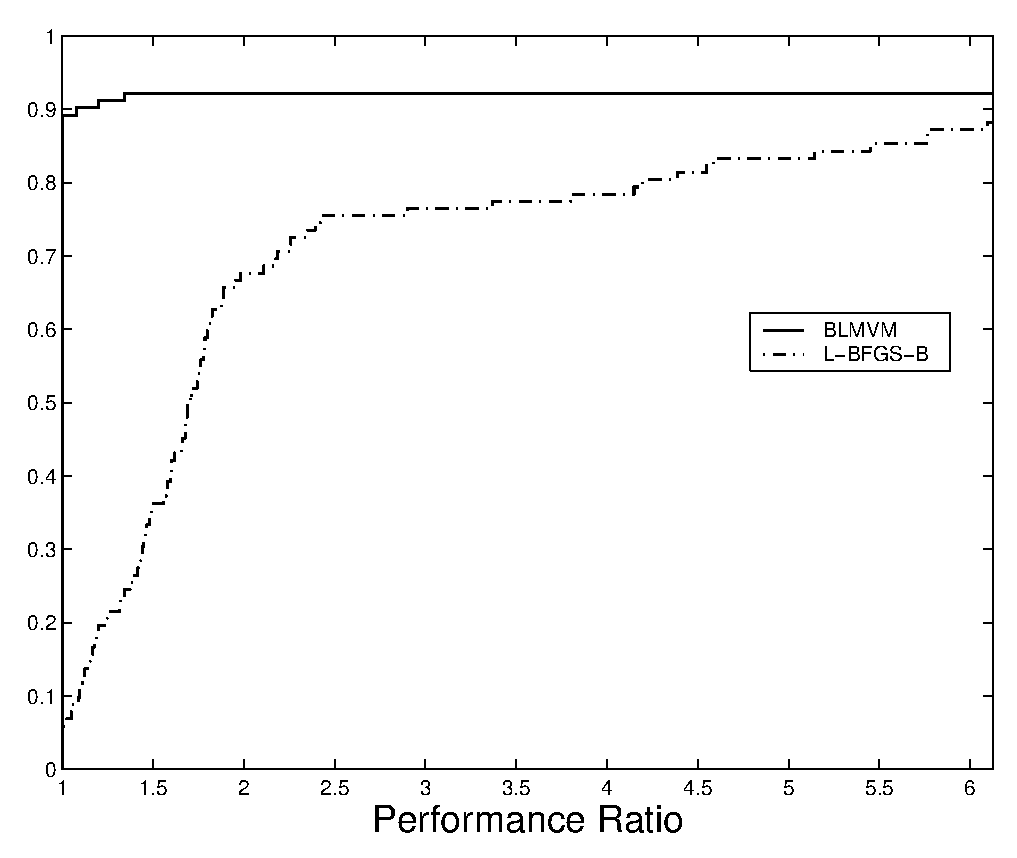
\includegraphics[width=0.45\textwidth,height=0.4\textwidth]{h1.eps}}
   \hskip 0.00\textwidth
   \subfigure[Function Evaluations]{
   \label{PFG}
   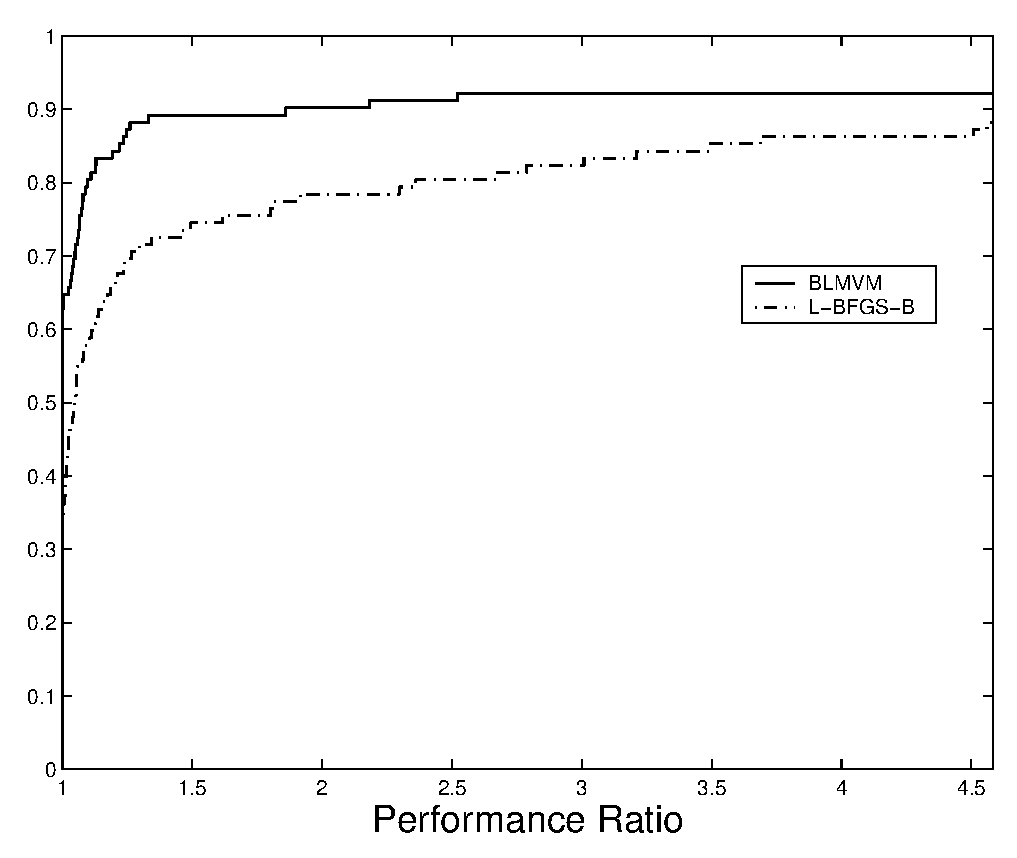
\includegraphics[width=0.45\textwidth,height=0.4\textwidth]{h2.eps}} \\
\label{figure3}
\end{center}
\end{figure}

We applied the performance profiling techniques introduced by Dolan
and Mor\'e\cite{dolan2} to
interpret the results.
Their profiles require a single statistic that measures the performance
of a solver on a problem.  We computed one profile using execution time
and another using the number of function and gradient evaluations.

To create these performance profiles, we first identify the best solver
for each  problem in the test suite.  
Then we compute the ratio of each solver's performance
versus the performance of the best solver.  A ratio of $1.0$ indicates
that the solver was at least as good as the other solvers on that problem
while a ratio greater than one indicates how much worse the solver performed
compared to the best solver.  
When a solver failed to find a solution satisfying the 
specified criteria, we set the ratio to $+\infty$.

Given these ratios, we define a function for each solver.  For every
number greater than or equal to one, this function is
defined to be the percentage of instances where the solver's performance
ratio is less than this number.  This cumulative distribution function
can be plotted for each solver.
The left side of the graph shows how often each solver was the best solver
and the right side of the graph show how often each solver successfully
found a solution.

Figures \ref{figure3} compare the performance of BLMVM to L-BFGS-B
using execution time and number of function evaluations. In both
algorithms, the function and gradient vector were evaluated in
the same routine.
The right side of each graph indicates the robustness of each algorithm
by the percentage of problems that
each algorithm successfully solved.  
Both algorithms fared well by solving about %90/%$ of
the problems to the prescribed accuracy.  BLMVM failed on 8 problems
while L-BFGS-B failed on 12 problems.

The left side of the graphs show the percentage of instances in which each
algorithm performed better than the other.  In terms of function
evaluations, BLMVM used fewer evaluations on about $60\%$ of the problems
while L-BFGS-B used fewer function evaluations on about $30\%$ of the problems.
In terms of execution time, BLMVM performed better on $90\%$ of the test suite,
while  L-BFGS-B used less time on only a few problems.

In addition, we found that when function evaluations were used a measure,
BLMVM performed L-BFGS-B by a factor of two on $15\%$ of the problems and
a factor of three on $10\%$ of the problems.   When execution time was used
as the measure, BLMVM performed L-BFGS-B by a factor of two on $25\%$ of the problems and
a factor of three on $15\%$ of the problems.
On average, BLMVM was about $40\%$ faster than
the competition.  

Since BLMVM uses fewer function evaluations on most problems, we feel that the
step direction used in BLMVM is better than the one used by  L-BFGS-B.  
In terms of execution time, BLMVM shows a
distinct advantage.  In all but a few cases, it found a solution
in less time.  These facts indicate that one iteration of the
BLMVM algorithm is usually cheaper that one iteration of L-BFGS-B.
Whereas L-BFGS-B first identifies a face in the feasible region and
then minimizes over that face, BLMVM always computes a step direction
in the full space.  By not explicitly working in a subspace,
BLMVM saves the time that other algorithms spend identifying it.
These features, and the use of the two-loop recursion instead of the compact
form, make the BLMVM algorithm efficient and relatively simple to implement.

\comment{
The fact that the number of evaluations is less indicates that our
step directions are better.  Even though the theorem only applies
to the when the iterates are on the optimal face, we are gradually
eliminating the effects of the gradient in the free variables.
}


\section{Scalability Using Multiple Processors}

To demonstrate the parallel efficiency of the algorithm,
we solved the obstacle problem from the MINPACK-2 test
suite using 1 - 512 processors.  
This benchmark is a variational problem over a two
dimensional region.  
It asks for the surface with the least area that satisfies a 
set of boundary conditions and lies above an obstacle within
the region. 
Given a two dimensional region ${\cD}$, an obstacle $v_L(x)$ defined on
that region, and boundary conditions $v_D (x)$,
the infinite dimensional version of this problem can be stated as

\[
\min \left \{ f(v) :
v \in H^1, \ v(x) = v_D (x) \ \ \forall  x \in \partial \cD, \ 
                v(x) \ge v_L (x) \ \ \forall  x \in \cD
\right \}
\]
where 
\[
f(v) = \int_{\cD} \sqrt{ 1 + \| \grad v(x) \|^2 } \; dx
\]

%\centerline {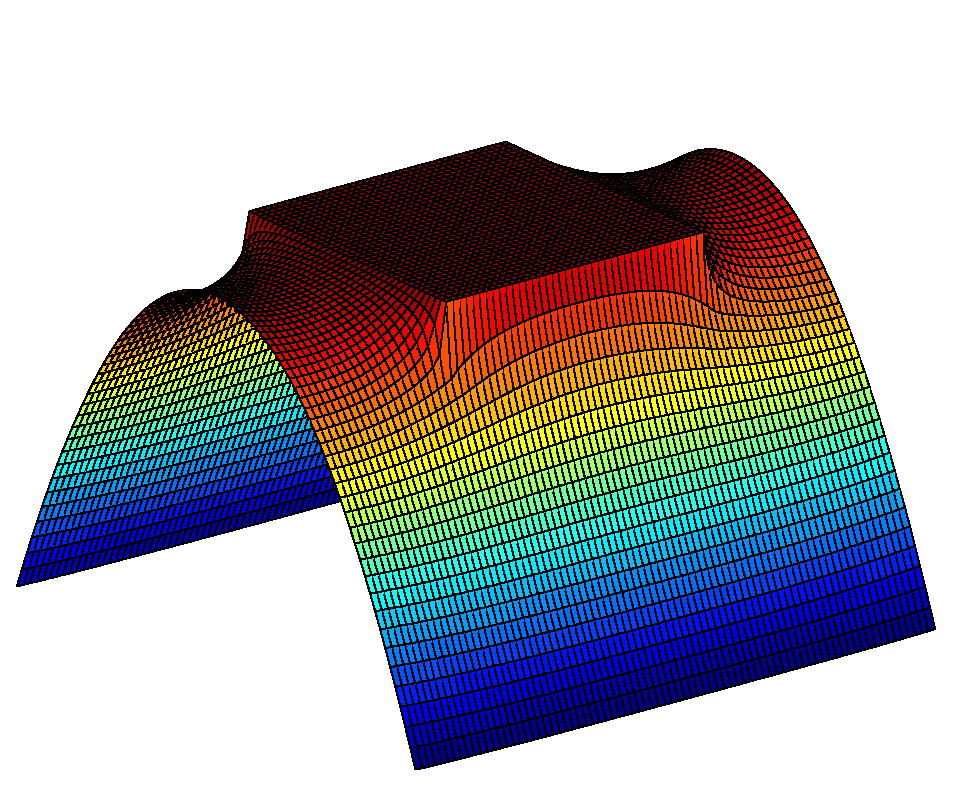
\includegraphics[height=2.1in]{../tutorials/images/mso.eps}}
\centerline {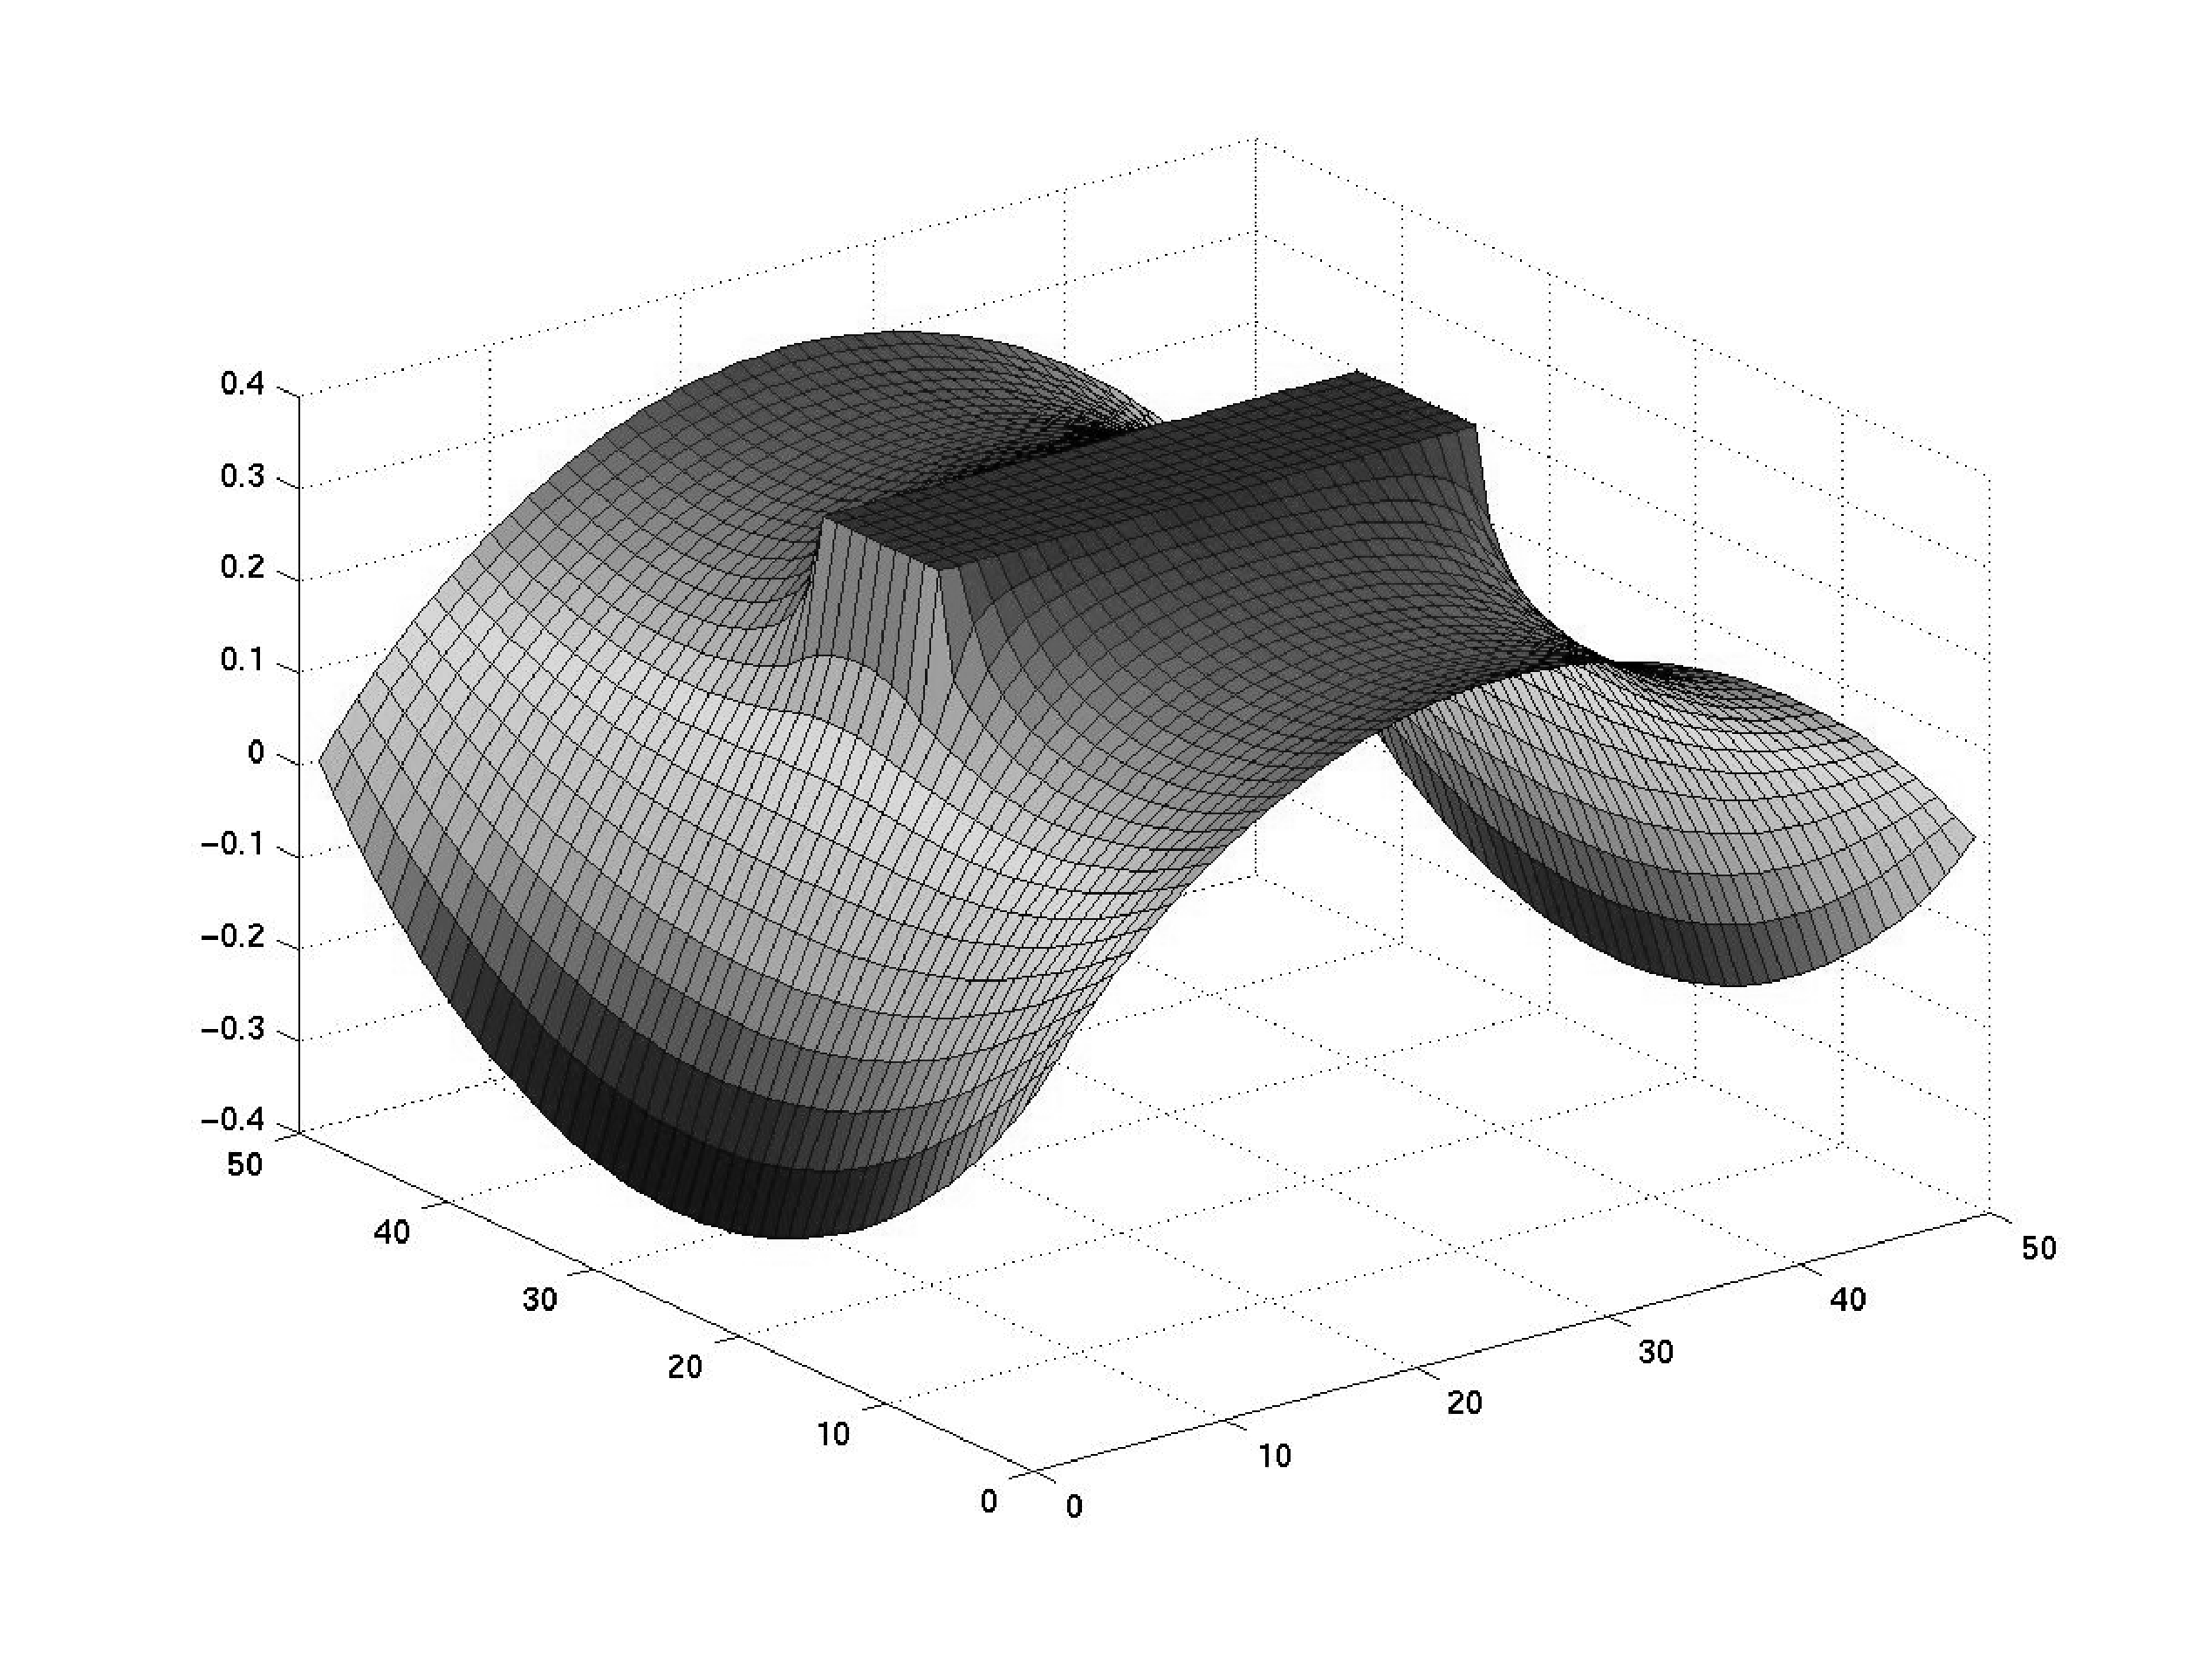
\includegraphics[height=3.1in]{surf5.ps}}

We prepared this problem for parallel computing 
using the grid management facilities of PETSc, 
which relies on MPI \cite{using-mpi} for all
communication between processors.
PETSc provides support for
discretizing the rectangular region ${\cD}$,
partitioning the surface into multiple regions and assigning
each processor to one these regions.  Each processor computes the surface
area of its region and the gradient of the objective value with respect to
the variables in its region.

These computations were performed on the Cray T3E supercomputer at the 
National Energy Research Scientific Computing Center (NERSC).
Each processor on this computer has 256 MB of RAM, and clock speed 
of 450 MHz, and a peak performance of  900 Mflops.  


Our first tests discretized the region into a $1600 \times 1600$ mesh,
which creates $2,560,000$ variables.  The obstacle was a rectangular
plate covered by the $640 \times 960$ mesh points in the middle of the
mesh.  The height of the plate was set to $0.2$.
The memory requirements of a problem
this large are so high that it exhausted the memory of the computer
when only four processors were used.  We solved the problem using as
few as 8 processors and as many as 512 processors.
Table 
\ref{routines} shows the number of iterations,
and seconds used to solve the problem in each test.
The table also indicates the
percentage of time spent in various parts of the algorithm.  The
time spent adding vectors is shown under the label {\tt AXPY}.
This category also includes time spent
copying vectors, projecting vectors, and performing other vector operations 
that do not require communication between processors.  The
{\tt Dot} column indicates the percentage of time spent performing vector
inner products and vector norms.  The column {\tt FG} shows the
percentage of time spent computing the function and gradient.

\begin{table}[bhpt]
\small
\begin{center}
\begin{tabular}{|cccccc|}
\hline
\multicolumn{1}{|c|}{Processors} &
\multicolumn{1}{c|}{BLMVM} &
\multicolumn{1}{c|}{Execution} &
\multicolumn{3}{c|}{Percentage of Time} \\
%\multicolumn{1}{|c|}{} \\
\multicolumn{1}{|c|}{Used}&
\multicolumn{1}{|c|}{Iterations}&
\multicolumn{1}{c|}{Time}&
\multicolumn{1}{c}{AXPY}&
\multicolumn{1}{c}{Dot} &
\multicolumn{1}{c|}{FG} \\
%\multicolumn{1}{c|}{FLOPS} \\

%\hline
%
%1 & 566 & 1226.0 & 29 & 9 & 62 & 36 \\
%2 & 690 & 736.9 & 29 & 9 & 62 & 74 \\
%4 & 559 & 305.9 & 29 & 8 & 63 & 144 \\
%8 & 550 & 172.6 & 26 & 8 & 66 & 251 \\
%16 & 570 &  78.6 & 28 & 11 & 60 & \\
%32 & 691 & 37.6 & & & & \\
%64 & 572 & 21.7 & 24 & 15 & 54 & \\
%128 & 695 & 14.7 & 24 & 20 & 55 & 3725 \\
%256 & 695 & 9.0 & 28 & 27 & 55 & 3725 \\
\hline

8 & 996 & 1083.8 & 31  & 9 & 60 \\ %& 256 \\
16 & 991 & 538.2 & 30 & 10 & 60 \\ %& 580 \\
32 & 966 & 267.7 & 29 & 11 & 60 \\ %& 1137 \\
64 & 993 & 139.5 & 27 & 13 & 60 \\ %& 2027 \\
128 & 987 & 72.4 & 25 & 15 & 60 \\ %& 3728 \\
256 & 996 & 39.2 & 26 & 18 & 56 \\ %& 8009 \\
512 & 1000 & 21.6 & 23 & 22 & 53 \\
\hline
\end{tabular}
\caption{Performance of BLMVM on Obstacle Problem.}
\label{routines}
\end{center}
\end{table}

Since more than $60\%$ of the execution time was spent
evaluating the function and gradient,
an efficient implementation of this routine is mandatory for good 
parallel performance.
Our function has a structure that allows an efficient parallel evaluation,
and its scalability is demonstrated by the fact that the percentage of
time spent in this routine did not increase with the number of processors.

The rest of the time was spent computing the BLMVM step direction and
projecting the new step into the feasible region.  Operations such as
scaling vectors, adding vectors,
copying the elements of one vector to another, and applying the projections 
$P$ and $G$  do not require any communication between processors.
These operations scale very well to more processors, and the percentage
of time spent in these operations declined as the number of processors 
increased.  The bottleneck in numerical computations involve
vector inner products and norms.  
These operations require communication between processors, whose overhead
degrades performance.
In this problem, the percentage of time spent in these operations 
more than doubled from $9\%$ to $22\%$.  

The overall efficiency of our implementation is shown in Figure \ref{G14}.
Each bar indicates the performance of BLMVM of each test relative to
the performance of BLMVM on eight processors.  
This number is the ratio of eight times the execution time using 
eight processors and the number of processors multiplied by the
time need to solve the problem using those processors.
Relative to the performance of BLMVM on this problem using eight processors,
the overall parallel efficiency using 256 processors was over $86\%$
and the overall parallel efficiency using 256 processors was over $78\%$.

In a second set of tests we solved obstacle problem using a mesh that was
refined according the number of processors used to solve the problem.
In these tests each processor owned $10,000$ variables.
The mesh was $100 \times 100$ when one processor was used and 
$1600 \times 1600$ when $256$ processors were used.  The length
and width of the obstacle were adjusted proportionately.  Since BLMVM
uses more iterations to solve problems with  finer meshes, we used
the rate of floating point operations as the measure of efficiency.
Figure \ref{G14chol} shows the average number of floating point operations
performed per second on each processor.  The problem used over $34$ MFlops when
one processor was used and that rate only decreased to about  $31$ MFlops when
when 256 processors were used.
Our parallel efficiency by this measure was over $90\%$.


\begin{figure}[ht]
\begin{center}
\caption{Parallel Efficiency of BLMVM on the Obstacle Problem.}
   \subfigure[Overall Implementation Efficiency]{
   \label{G14}
   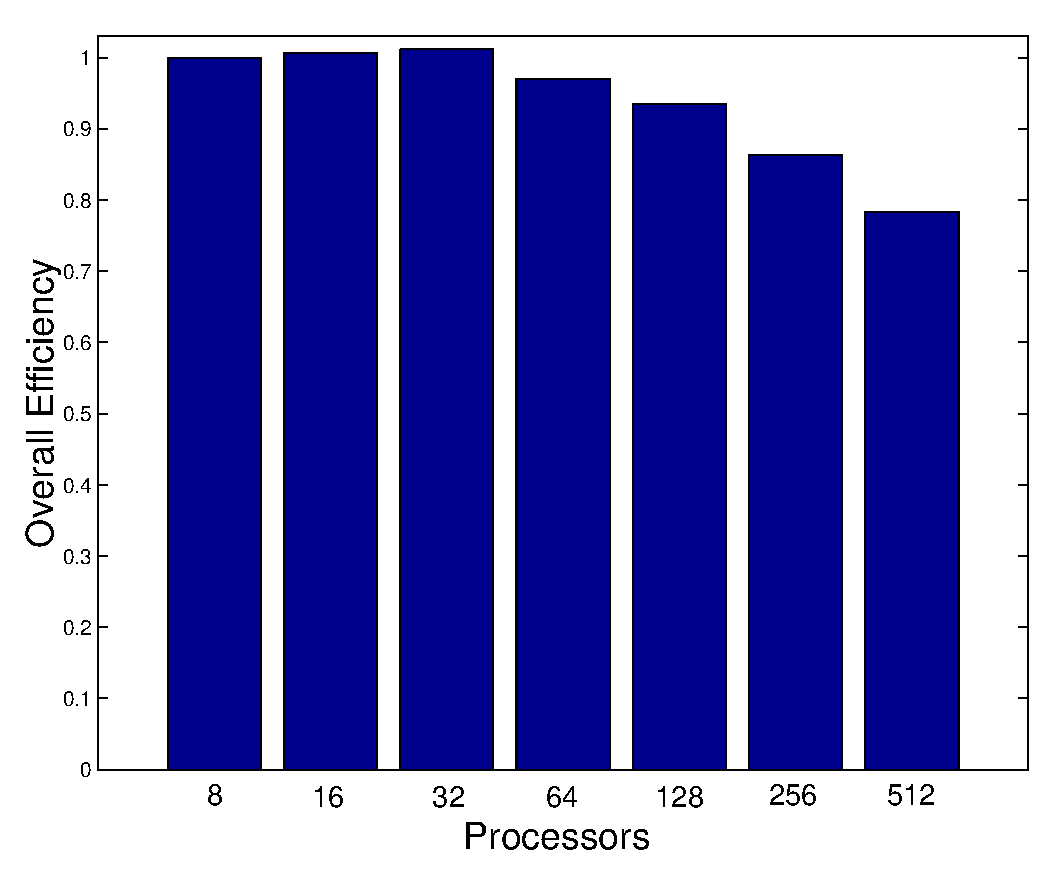
\includegraphics[width=0.45\textwidth,height=0.4\textwidth]{f4.eps}}
   \hskip 0.00\textwidth
   \subfigure[Floating Point Efficiency]{
   \label{G14chol}
   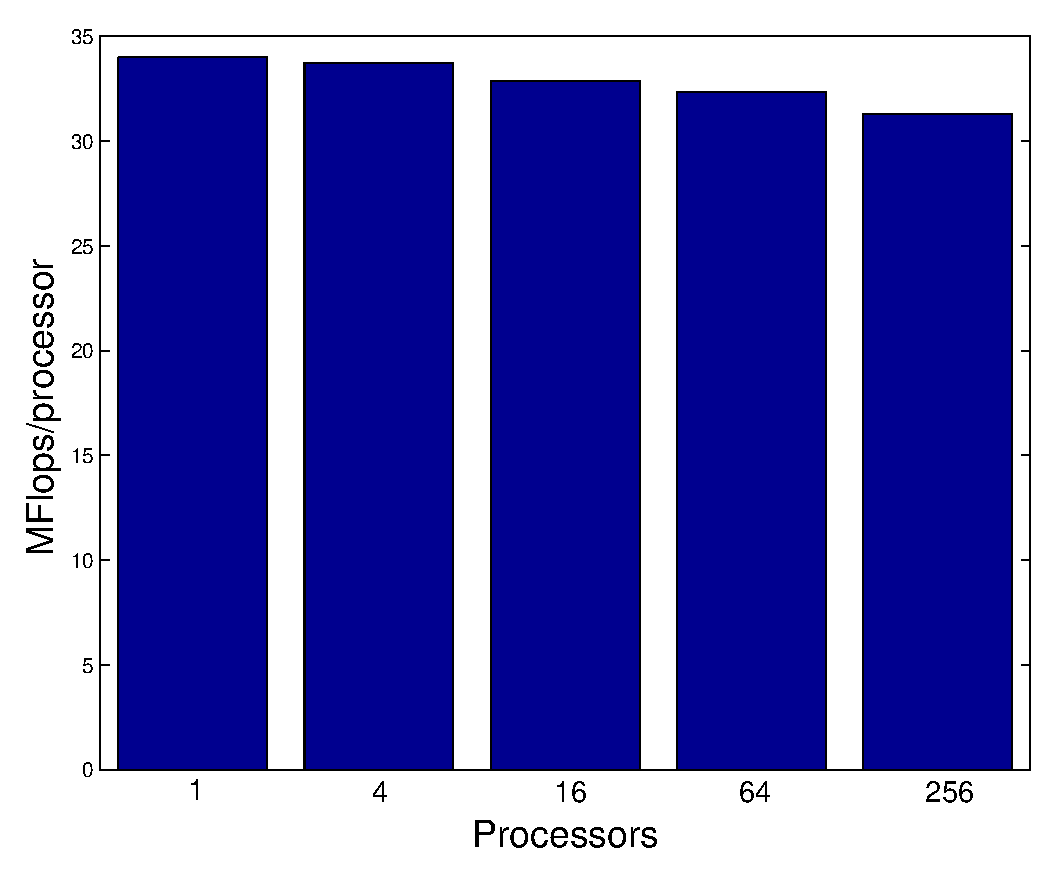
\includegraphics[width=0.45\textwidth,height=0.4\textwidth]{f3.eps}} \\
\label{figure2}
\end{center}
\end{figure}


\section{Conclusion}

We have described a robust and efficient method
bound constrained optimization that requires only 
function and gradient evaluations from the objective function. 
Its limited storage requirements make it well
suited for large optimization problems.  
On some large problems, the algorithm can also compute a
solution in parallel with high level of efficiency.
Against other solvers in its class, numerical experiments showed
that it performed very well.

Our implementation of this algorithm is available in 
the Toolkit for Advanced Optimization (TAO).  
The TAO project \cite{tao-web-page,tao-user-ref}
focuses on the design and implementation of
component-based optimization software for the
solution of large-scale optimization applications.
Its design enables connection to lower-level
support (parallel vectors, sparse matrix data
structures, preconditioners, solvers) provided in toolkits such as
PETSc,
and thus we are able to build on top of these toolkits
instead of having to redevelop code. 
Initial work in TAO
has centered on the development of solvers for 
unconstrained and bound-constrained minimization and
nonlinear least squares.


%\input{cg}

\bibliographystyle{siam}

\bibliography{../tao,%
/home/more/papers/bibs/opt80,%
/home/more/papers/bibs/opt90}%

\end{document}

